\documentclass{article}
\usepackage[utf8]{inputenc}
\usepackage[italian]{babel}
\usepackage[T1]{fontenc}
\usepackage{amsmath}
\usepackage{listings}
\usepackage{color}
\usepackage{graphicx}
\usepackage{enumerate}
\usepackage{adjustbox}
\usepackage{mathtools}
\usepackage{amssymb}
\usepackage{float}
\usepackage{hyperref}
\graphicspath{ {./images/} }

\newcommand{\norm}[1]{\left\lVert#1\right\rVert_2}

\definecolor{dkgreen}{rgb}{0,0.6,0}
\definecolor{gray}{rgb}{0.5,0.5,0.5}
\definecolor{mauve}{rgb}{0.58,0,0.82}

\lstset{emph={getCorrectBit, varOne, varZero, attackerdevice, victimdevice, getrandbits, NUM_TESTS, TimingAttack, EEA, fastExp, testMR, primeGen, __init__, encrypt, decrypt, decryptCRT}, emphstyle=\color{mauve},
        emph={[2]append}, emphstyle={[2]\color{blue}}
        }

\lstset{frame=tb,
  language=Python,
  aboveskip=3mm,
  belowskip=3mm,
  showstringspaces=false,
  columns=flexible,
  basicstyle={\small\ttfamily},
  numbers=none,
  numberstyle=\tiny\color{gray},
  keywordstyle=\color{blue},
  commentstyle=\color{dkgreen},
  stringstyle=\color{mauve},
  breaklines=true,
  breakatwhitespace=true,
  tabsize=3
}


\title{Esercizi Set 3}
\author{Lorenzo Macchiarini}
\date{4 Giugno 2021}

\begin{document}

\maketitle

\section{Esercizio 2.2: Strategie e Codici}

\begin{enumerate}[(a)]
    \item In Figura \ref{fig:Tree} possiamo vedere un esempio di albero di pesate per stimare correttamente l'azione compiuta da A. Notiamo come il numero di foglie è 11, ovvero $2n+1$ con $n=5$, in quanto ci sono 2 possibili azioni svolte da B per ogni moneta (sostituzione con una più pesante o una più leggera) e l'azione "nessuna sostituzione svolta". Possiamo notare inoltre come tale albero non sia completo perché non tutti i rami della radice hanno il massimo numero di nodi.
    \begin{figure}[h]
    \centering
    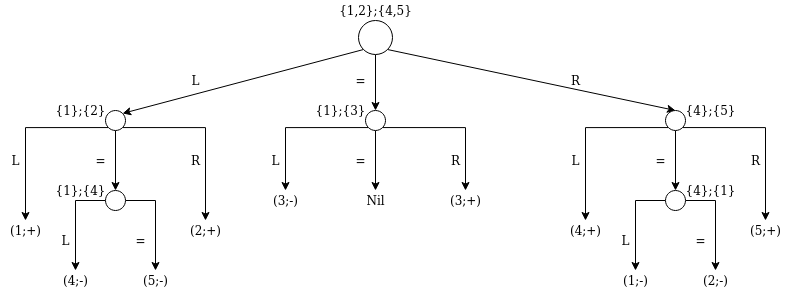
\includegraphics[width=12cm]{images/Diagram.png}
    \caption{Albero ternario che rappresenta le possibili pesate da svolgere nel caso in cui si abbiano 5 monete. La pesata fra due set di monete è rappresentata da \textit{\{set1\};\{set2\}}, la stima di quale azione è stata compiuta è rappresentata da \textit{(moneta;azione)}}
    \label{fig:Tree}
    \end{figure}
    \item In questo esempio ho che:
    \begin{itemize}
        \item Il numero di pesate massimo è 3;
        \item Il numero di pesate medio è: 
        \begin{equation}
            \sum_{f \in foglie}altezza(f)*prob(f)=\left(3 \times \frac{1}{11} \right) \times 4 + \left(2 \times \frac{1}{11} \right) \times 7 = 2.36
        \end{equation}
        Tale valore è diverso da 3 poiché l'albero non è completo e quindi non tutte le foglie hanno altezza massima.
    \end{itemize}
    \item Chiamiamo $k$ il numero massimo di pesate con cui si riesca a conoscere completamente $X$. Per definizione abbiamo che $H(X|Y_1, ... , Y_k) = 0$ perché le $k$ pesate determinano completamente $X$. Sviluppo quindi tale formula:
    \begin{equation}
    \begin{split}
        H(X|Y_1, ... , Y_k) &= H(X,Y_1, ... , Y_k) - H(Y_1, ... , Y_k)\\
                            &= H(Y_1, ... , Y_k|X) + H(X) - H(Y_1, ... , Y_k)
    \end{split} 
    \end{equation}
    In questo caso ho applicato solamente la Chain Rule sviluppando $H(X|Y)$ e $H(Y|X)$. Analizzando $H(Y_1, ... , Y_k|X)$ e applicando lo stesso ragionamento svolto per $H(X|Y_1, ... , Y_k)$, notiamo che $H(Y_1, ... , Y_k|X) = 0$ in quanto la conoscenza di $X$ determina univocamente i valori delle pesate svolte. Quindi ottengo:
    \begin{equation}
    \begin{split}
        H(X|Y_1, ... , Y_k) &= H(X) - H(Y_1, ... , Y_k)\\
                          0 &= H(X) - H(Y_1, ... , Y_k)\\
                          H(X) &= H(Y_1, ... , Y_k)
    \end{split} 
    \end{equation}
    Analizzo quindi i due termini:
    
    \begin{itemize}
        \item Per il corollario della Chain Rule ottengo:
        \begin{equation}
            H(Y_1, ... , Y_k) \leq \sum^{k}_{i=1}H(Y_i)
        \end{equation}
        Ed in particolare i due termini sono uguali se e solo se le pesate sono indipendenti.\\
        Sviluppando la definizione di entropia per ogni $Y_i$ , ricordando che prende valori fra $1$ e $3$ in modo uniformemente distribuito con probabilità $\frac{1}{3}$, otteniamo:
        \begin{equation}
            H(Y_1, ... , Y_k) \leq\sum^{k}_{i=1}H(Y_i)=\sum^{k}_{i=1} \sum^{3}_{j=1} \frac{1}{3} \lg(3) = k \lg(3)
        \end{equation}
        \item Per la definizione di entropia e considerando che lo spazio dei possibili valori di X ha cardinalità $2n+1$, ognuno dei quali ha la stessa probabilità $\frac{1}{2n+1}$:
        \begin{equation}
            H(X) = \sum^{2n+1}_{i = 1} \frac{1}{2n+1}\lg(2n+1) = \lg(2n+1)
        \end{equation}
    \end{itemize}   
    Aggregando quindi tali osservazioni otteniamo che:
    \begin{equation}
        \begin{split}
            H(Y_1, ... , Y_k) &= H(X) \\
            k\lg(3)&\geq \lg(2n+1) \\
            k &\geq \frac{\lg(2n+1)}{\lg(3)}\\
            k &\geq \log_3(2n+1) 
        \end{split}   
    \end{equation}
    Otteniamo quindi un limite inferiore per il numero massimo di pesate necessarie per stimare correttamente $X$. Possiamo inoltre notare come il risultato sarebbe stato lo stesso nel caso in cui avessimo considerato $\log_3$ anziché $\log$ all'interno delle entropie calcolate.\\
    Confrontando tale risultato con il caso di 5 monete otteniamo che $k=3$ e $ \log_3(11)=2.18$, quindi $3 \geq 2.18$.
    \item Come riportato nelle note all'esercizio possiamo considerare l'albero ternario come un albero corrispondente ad un codice istantaneo con tre rami per ogni nodo anziché due. Applicando il \textit{primo teorema di Shannon} e utilizzando l'entropia $H_3$, possiamo esprimere il numero medio di pesate come la lunghezza media dei rami dell'albero:
    \begin{equation}
        L(C) \geq H(X) = H_3\left(\frac{1}{2n+1},...,\frac{1}{2n+1}\right)
    \end{equation}
    Con la distribuzione dei valori di $X$ uniforme ed uguale a $\frac{1}{2n+1}$. Sviluppando quindi otteniamo,
    \begin{equation}
        L(C) \geq H_3\left(\frac{1}{2n+1},...,\frac{1}{2n+1}\right) = \sum^{2n+1}_{i = 1} \frac{1}{2n+1}\log_3(2n+1) = \log_3(2n+1)
    \end{equation}
    Confrontando tale risultato con l'esempio con 5 monete otteniamo che: $L(C)=2.36$ e $ \log_3(11)=2.18$, quindi $2.36\geq 2.18$.
\end{enumerate}

\section*{Esercizio 3.2 Codici di Huffman}
L'algoritmo di Huffman permette di creare un codice prefix free a partire da un alfabeto e la sua relativa distribuzione di probabilità. L'algoritmo viene eseguito bottom-up, ovvero viene creato un albero binario che associa ad ogni nodo una codeword a partire dagli elementi dell'alfabeto e dalle loro frequenze. Possiamo definire due fasi di esecuzione dell'algoritmo:
\begin{enumerate}
    \item La prima in cui vengono aggregati i nodi per creare l'albero:
    \begin{itemize}
        \item Vengono create le foglie dell'albero, una per ogni carattere dell'alfabeto, a cui vengono associate per ognuna la probabilità di uscita del carattere corrispondente;
        \item Fino a quando non viene ottenuta la radice viene creato un nuovo nodo interno all'albero che aggrega i due nodi (o foglie) non ancora esplorati che hanno le probabilità minori fra tutti quelli da esplorare. Il nodo risultante avrà come probabilità associata la somma delle due probabilità dei due nodi trovati.
        \item La radice è l'ultimo nodo generato ed avrà probabilità 1.
    \end{itemize}
    \item La seconda in cui, una volta creato l'albero, viene associata una codeword ad ogni carattere dell'alfabeto:
    \begin{itemize}
        \item La fase parte dalla radice, a cui viene associata la stringa vuota;
        \item Per ogni nodo successivo esplorato viene assegnata la stringa del predecessore a cui viene aggiunto $0$ o $1$ in modo indifferente.
        \item Al termine dell'algoritmo quindi avremo ottenuto un codice in cui ad ogni elemento dell'alfabeto (forglia) viene associata una codeword.
    \end{itemize}
\end{enumerate}
Nell'implementazione sviluppata ho implementato una funzione \textit{huffman(input)} in cui l'input atteso è una lista di coppie \textit{("elemento alfabeto",probabilità)}. Ognuna di queste coppie andrà a determinare le foglie dell'albero. Ho rappresentato ogni nodo con un dizionario python in cui sono presenti:
\begin{lstlisting}
{
    "symbol": "a", # elemento corrispondente dell'alfabeto (!= " " solo per le foglie)
    "probability": 0.1, # probabilita' del nodo
    "value": 110, # valore finale associato al nodo
    "components": [] # lista contenente la coppia di nodi figli
}
\end{lstlisting}
Quindi inizialmente vengono generate le foglie necessarie con i relativi simboli e probabilità corrette. Ogni nodo creato è salvato nel dizionario \textit{nodes} in cui ad ogni nodo è associato un id, mentre i nodi che devono essere ancora esplorati sono riportati in \textit{edge}. Inizialmente tutte le foglie sono aggiunte sia a \textit{nodes} sia a \textit{edge} e anche ad un dizionario che memorizza quali sono le foglie iniziali (\textit{initial}).
\begin{lstlisting}
def huffman(input):
    nodes = {}
    edge = []
    currentID = 0
    initial = {}
    for inp in input:
        node = {}
        node["symbol"] = inp[0]
        node["probability"] = inp[1]
        node["value"] = None # valore nullo aggiornato in seguito alla computazione finale
        node["components"] = [] # le foglie non hanno figli
        initial[currentID] = node
        nodes[currentID] = node
        edge.append(node)
        currentID += 1
\end{lstlisting}
Una volta inizializzato \textit{edge}, iteriamo fino a quando non viene trovata la radice (ovvero fino a quando \textit{edge} ha lunghezza $>= 2$. Ad ogni passo vengono trovati i due nodi in \textit{edge} che hanno probabilità minori e viene generato un nuovo nodo con probabilità la somma delle due probabilità e con figli i due nodi trovati. Quindi vengono rimossi da \textit{edge} i due nodi e aggiunto il nuovo nodo a \textit{nodes} e ad \textit{edge}.
\begin{lstlisting}
    while(len(edge) > 1):
        # trova el1 e el2 i nodi con probabilita' minori
        min1 = 1
        min2 = 1
        el1 = None
        el2 = None
        for e in edge:
            if(e["probability"] < min2):
                el2 = e
                min2 = e["probability"]
                if(min2 < min1):
                    min1, min2 = min2, min1
                    el1, el2 = el2, el1
        # creo il nuovo nodo ed aggiorno le liste e dizionari
        newNode = {}
        newNode["probability"] = round(min1 + min2, 4)
        newNode["components"] = [el1, el2]
        newNode["value"] = None
        edge.remove(el1)
        edge.remove(el2)
        nodes[currentID] = newNode
        edge.append(newNode)
        currentID += 1
\end{lstlisting}
La prima fase di creazione dell'albero quindi è conclusa. Per assegnare i valori del codice ad ogni nodo inizialmente viene settato il codice della radice alla stringa vuota. Partendo dalla radice analizzo i figli di ogni nodo utilizzando il vettore \textit{toExpand}, in cui inserisco i soli nodi a cui è stato appena settato il codice. L'ultima iterazione si ha quando \textit{toExpand} è vuoto.
Per ogni nodo presente in \textit{toExpand} modifico il codice dei suoi figli copiando il codice del nodo padre (il nodo corrente) e aggiungendo $0$ o $1$ a seconda della posizione del figlio nella lista, ovvero in base a quale dei due figli ha la probabilità minore. Quindi rimuovo da \textit{toExpand} il nodo appena analizzato ed aggiungo i due nuovi nodi. Se il nodo analizzato fosse una foglia non viene analizzato nessun altro nodo e viene unicamente rimosso il nodo da \textit{toExpand}.\\
\begin{lstlisting}
    edge[0]["value"] = ""
    toExpand = [edge[0]] # inizializzato con il nodo radice
    while(len(toExpand) != 0):
        currentExp = toExpand # non aggiorno dinamicamente i nodi da analizzare
        for el in currentExp:
            for i in range(len(el["components"])):
                el["components"][i]["value"] = el["value"] + str(i)
                toExpand.append(el["components"][i])
            toExpand.remove(el)
\end{lstlisting}
Il modo in cui analizzo nuovi nodi è di tipo breadth first anzichè depth first in quanto ad ogni iterazione analizzo i soli nodi che erano presenti in \textit{toExpand} all'iterazione precedente. \\
Al termine di entrambe le fasi ho che i nodi foglia contengono sia i simboli dell'alfabeto iniziale definito dall'utente sia le codeword generate. Per rendere più semplice la codifica e decodifica del codice viene ritornata una specie di dizionario cartaceo in cui ho memorizzato sia la traduzione da alfabeto a codice sia da codice ad alfabeto.
\begin{lstlisting}
    for i in initial: # ciclo sui nodi iniziali aggiornati con i codici
        retValue["bin_to_chr"][initial[i]["value"]] = initial[i]["symbol"]
        retValue["chr_to_bin"][initial[i]["symbol"]] = initial[i]["value"]
\end{lstlisting}    
La funzione di \textit{encode} prende in ingresso il dizionario da alfabeto a codewords e la stringa da codificare. La codifica avviene codificando ogni lettera della stringa "traducendola" utilizzando il dizionario in input.
\begin{lstlisting}
def encode(alphabet, string):
    encoded = ""
    for s in string:
        encoded += alphabet[s]
    return encoded
\end{lstlisting}
La funzione di \textit{decode} prende in ingresso il dizionario da codewords ad alfabeto e la stringa di bit da decodificare. Poiché il codice da decodificare sappiamo essere prefix free, ogni codeword del codice non è contenuta nella prima parte di altre codewords. Quindi la decodifica avviene scansionando la stringa di bit da sinistra verso destra e riconoscendo blocchi di bit corrispondenti a codewords. La scansione avviene analizzando i blocchi di bit che non sono stati ancora associati a nessun carattere. Il blocco corrente non ancora associato a nessuna codeword è \textit{currentString}. Al bit successivo analizzato nella stringa in input verifico se \textit{currentString+bit} è una codeword o meno; se lo fosse aggiungo il carattere corrispondente alla stringa da ritornare e resetto \textit{currentString}.\\
\begin{lstlisting}
def decode(code, binary):
    finalString = ""
    currentString = ""
    for el in binary:
        if(currentString+el in code):
            finalString += code[currentString+el]
            currentString = ""
        else:
            currentString += el
    return finalString
\end{lstlisting}
Per testare il corretto funzionamento degli algoritmi ho utilizzato tre tipi di alfabeti e "dizionari" diversi:
\begin{itemize}
    \item Un alfabeto di 4 lettere e relative frequenze di test;
    \item Gli alfabeti italiano e inglese con le relative distribuzioni di probabilità di ogni lettera;
    \item Due dizionari di 4 lettere ciascuno a cui è associato un codice prefix free stabilito e non generato con l'algoritmo di Huffman.
\end{itemize}
La codifica e decodifica avviene utilizzando il dizionario scelto \textit{usedDictionary} e una stringa generica \textit{string}.
\begin{lstlisting}
# dizionario di test con codice prefix free non Huffman
usedDictionary = {'chr_to_bin': {'a': '00', ... , 'o': '11'}, 
                    'bin_to_chr': {'00': 'a', ... , '11': 'o'}}
string = "abaco"
encoded = encode(usedDictionary["chr_to_bin"],string)
decoded = decode(usedDictionary["bin_to_chr"],encoded)
\end{lstlisting}    
Come atteso, sia la codifica che la decodifica danno sempre esito corretto nel caso in cui il codice sia prefix free. Ho verificato anche che il codice soddisfi:
\begin{equation}
    H(p) \leq L_p(c) < H(p)+1
\end{equation}
con le funzioni:
\begin{lstlisting}
def entropy(alphabet):
    value = 0
    for a in alphabet:
        value -= a[1]*math.log2(a[1])
    return value
\end{lstlisting}
\begin{lstlisting}
def meanLength(dict, alphabet):
    value = 0
    for a in alphabet:
        if(a[0] in dict):
            value += a[1]*len(dict[a[0]])
    return value
\end{lstlisting}
ed in tutti e tre i casi di generazione del codice ciò è verificato.
\\
Dai test svolti possiamo notare anche come l'implementazione sia concorde a quanto atteso, ovvero che il codice generato dall'algoritmo di Huffman su una particolare distribuzione è quello con lunghezza media del codice $L_p(c)$ minore:
\begin{itemize}
    \item Se il codice utilizzato è molto piccolo (4 lettere) la codifica ottenuta sarà di lunghezza molto minore rispetto ad uno più grande (26 lettere). Infatti la lunghezza della codifica di \textit{"abaco"} con il dizionario composto da \textit{a, b, c, o} è 10 mentre quella con un dizionario di tutte le lettere dell'alfabeto con distribuzione italiana delle lettere è 21.
    \item Se il codice utilizzato è quello generato dalle frequenze di una certa lingua (italiano), la lunghezza di un testo della stessa lingua codificato con tale codice sarà minore rispetto ad uno generato con un codice derivante da frequenze di un'altra lingua (inglese). Per svolgere tale test ho codificato con entrambi i codici la prima frase delle rispettive pagine Wikipedia riguardo all'analisi delle frequenze \href{https://it.wikipedia.org/wiki/Analisi_delle_frequenze}{italiana} e \href{https://en.wikipedia.org/wiki/Frequency_analysis}{inglese} e ho ottenuto:
    \begin{itemize}
        \item Per il testo italiano le lunghezze delle codifiche sono: 1011 per il codice italiano e 1074 per quello inglese;
        \item Per il testo inglese le lunghezze delle codifiche sono: 768 per il codice italiano e 723 per quello inglese.
    \end{itemize}
\end{itemize}

\end{document}
